\subsection{Stochastic Volatility}\label{ssec:stochastic_volatility}

\begin{figure*}[t]
    \centering
    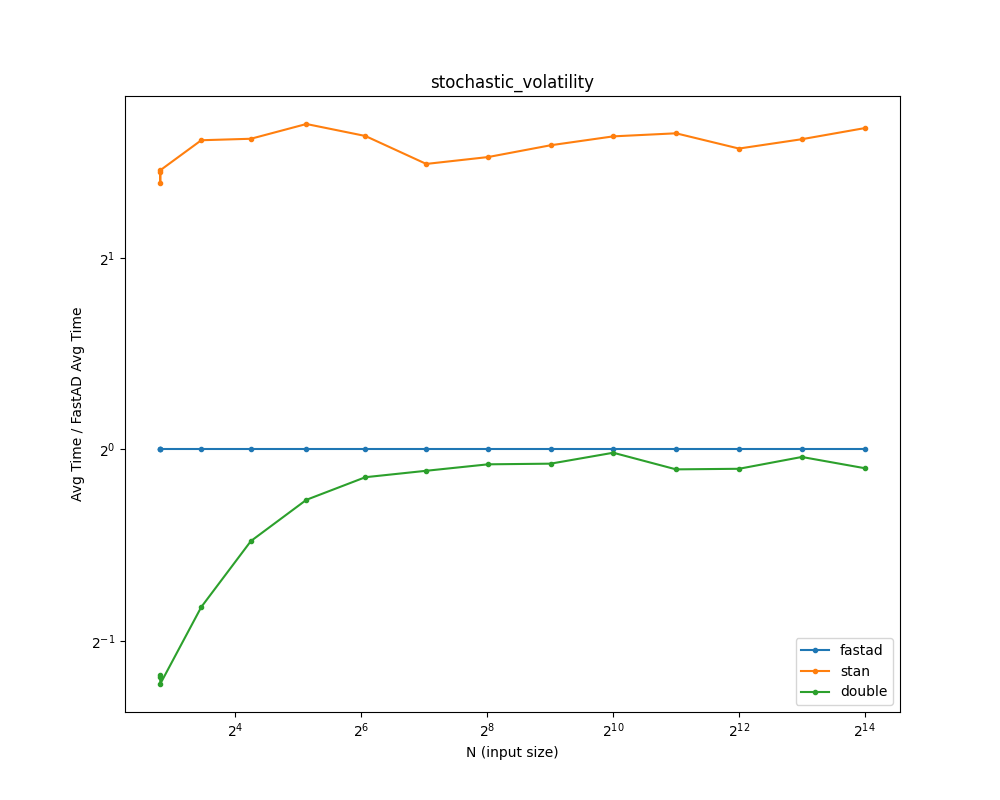
\includegraphics[width=0.8\textwidth]{figs/stochastic_volatility_fig.png}
    \caption{%
        Stochastic volatility benchmark of Stan against FastAD 
        plotted relative to FastAD average time.
    }\label{fig:stochastic_volatility}
\end{figure*}

This section marks the second and last macro-benchmark example.
We consider the following stochastic volatility model 
taken from the Stan user guide~\cite{stan-rm:2018}:
\begin{align*}
    y &\sim N(0, e^{h}) \\
    h_{std} &\sim N(0, 1) \\
    \sigma &\sim Cauchy(0,5) \\
    \mu &\sim Cauchy(0,10) \\
    \phi &\sim Unif(-1, 1) \\
    h &= h_{std} \cdot \sigma \\
    h[0] &= \frac{h[0]}{\sqrt{1 - \phi^2}} \\
    h &= h + \mu \\
    h[i] &= \phi \cdot (h[i-1] - \mu),\, i > 0
\end{align*}
The target function is the log of the joint probability density function (up to a constant)
and we wish to differentiate it with respect to $h_{std}, h, \phi, \sigma, \mu$.
Fig.~\ref{fig:stochastic_volatility} shows the benchmark results.

FastAD outperforms Adept by $2$ times and Stan by $ 2.6$ times for the largest $N$.
The trend seems to stabilize starting from $N = 2^{10}$.
It is interesting to see that FastAD actually performs better than the baseline
for moderate to large $N$ values.
For a complicated model as such, there are many opportunities for FastAD to cache certain
evaluations for constants as mentioned in Section~\ref{ssec:compile-time-opt} 
and~\ref{ssec:normal_log_pdf}.
In particular, the exponential function $ e^h$ reuses its forward-evaluated result,
and many log-pdfs cache the log of its parameters such as 
$\log(\sigma)$ in the Normal log-pdfs 
and $\log(\gamma)$ in the Cauchy log-pdfs 
($\sigma, \gamma$ are the second parameters of their respective distributions, 
which are constant in this model).
Note that this caching is automatically done in FastAD, 
which would be tedious to manually code for the baseline.
Hence, this shows that due to automatic caching, 
FastAD forward and backward-evaluation combined 
can be faster than a manually-written forward evaluation only, 
which puts FastAD at an optimal performance.
